\subsection{Uniform boundary weights hide an extensive thermal ledger}
\label{sec:stars-12}

An exact full-port example makes the distinction between equilibrium
elimination and microscopic history particularly sharp. For
$s\in\{-1,1\}^4$ let the eight rays be
$\mathcal P=\{(1,p_2,p_3,p_4):p_j=\pm1\}$. Couple $k$ independent
hidden layers by
\begin{equation}
 H(s,h)=-J\sum_{\ell=1}^k\sum_{p\in\mathcal P}h_{\ell,p}\,p\cdot s,
 \qquad x=\beta J>0.
\end{equation}
For every $s$, the eight magnitudes $|p\cdot s|$ are $4$ once, $2$ four
times and $0$ three times. Summing all hidden spins therefore gives
\begin{equation}
 Z_s=[256\cosh(4x)\cosh^4(2x)]^k,\qquad
 Z=16Z_s,\quad\pi_s=1/16.
\label{eq:star-partition-12}
\end{equation}
The normalized boundary equilibrium is independent of $k$. Its absolute
partition function, energy and entropy are not.\samref{REF12_THREE}

With unit attempts at each visible site and any fixed positive hidden
attempt rates, let $p(h)=\pi(h\mid s)$ and $q(h)=\pi(h\mid t)$ on
neighboring boundary masks. Equal boundary partitions and detailed balance
give projected edge rate $\Omega_k/2$, where
\begin{equation}
 \Omega_k=2\sum_h\frac{p(h)q(h)}{p(h)+q(h)}.
\end{equation}
Every edge has this multiplier by the signed-ray symmetry. Cauchy and
arithmetic--geometric mean bound it by the Hellinger affinity:
\begin{equation}
 h(x)^{2k}\le\Omega_k\le h(x)^k,\qquad
 h(x)=\frac{\cosh^2(3x)\cosh^6x}{\cosh(4x)\cosh^4(2x)}.
\end{equation}
For $x>0$, $k>0$, $0<h,\Omega_k<1$; $x=0$ or $k=0$ gives
$\Omega=1$. The statement concerns the instantaneous projected
generator. It does not identify the full microscopic semigroup.

For the visible spin $f=s_0$ and positive generator $A=-L$, the heatbath
complement at that site is an orthogonal projection in $L^2(\pi)$.
All other site complements kill $f$. Thus its spectral moments satisfy
\begin{equation}
 \mu_1=\langle f,Af\rangle=\Omega_k,\qquad
 \mu_2=\|Af\|^2=\Omega_k,
\end{equation}
and its rate spectral variance is $\Omega_k(1-\Omega_k)>0$.
The projected independent-bit clock has zero binary three-time conditional
information; the microscopic source has positive two-wait memory.
The invariant dispersion $1/\Omega_k-1$ survives a common clock rescaling.

At $x=\log2/2$, full enumeration visits all 4096 states for one layer.
It gives $Z_{\rm layer}=10625/8$, $Z=21250$, ground energy $-12J$ and
degeneracy 128. The exact layer multipliers, to displayed precision, are
\begin{equation}
\begin{aligned}
 \Omega_1&=.5442139601408111,&\Omega_2&=.3273194372007378,\\
 \Omega_3&=.2043615579016519,&\Omega_4&=.1302972507097655.
\end{aligned}
\end{equation}
Their full rational values are retained with the report. Differentiating
the complete partition at fixed $J$ gives
\begin{align}
 E/J&=-k[4\tanh4x+8\tanh2x],\\
 C_V/k_B&=k[(4x)^2\operatorname{sech}^2(4x)
                     +4(2x)^2\operatorname{sech}^2(2x)].
\end{align}
At this rational point $E/J=-708k/85$ and
\begin{equation}
 S(s,h)=4\log2+k\{\log(10625/8)-(354/85)\log2\}.
\end{equation}
The conditional Gibbs entropy and calorimetric ledger agree. The hidden
free-energy contribution relative to uncoupled spins is
$-k\beta^{-1}\log[\cosh4x\cosh^4(2x)]$. Boundary normalization cannot
erase it. No physical temperature, attempt rate, calorimeter or reusable
preparation/reset payment is fixed by this identity.

\subsection{A sharp rare-cell coefficient and the optimal layer count}
\label{sec:rare-cell-12}

For the stated reversible binary observation, the short-wait law is
\begin{equation}
 I(t,s)=\frac{ts}{4}\{b\log(b/a^2)-b+a^2\}
                 +O(ts(t+s)),\qquad b=\alpha a.
\end{equation}
The rare double-change cell requires this expansion; a regular-cell
quadratic approximation alone misses its leading term. At unit observed
attempt rate, $b=a$ and the coefficient is
\begin{equation}
 C(a)=\tfrac14a(-\log a-1+a),\qquad0<a\le1.
\end{equation}
Its derivative has the sign of $g(a)=-\log a-2+2a$.
$g$ decreases to $1/2$, increases thereafter, is negative at $1/2$ and
vanishes at one. Hence it has one interior root, the unique global maximum
of $C$. The certified intervals are
\begin{align*}
 a_*&\in[.20318786997997,.20318786998000],\\
 C_*&\in[.04047563986824320,.04047563986824766].
\end{align*}
Global concavity is unnecessary and false: $C''(3/4)=1/6>0$.

At the fixed eight-star rational dictionary above,
$C(\Omega_3)=.0404751384244456948686\ldots$, a fraction in
$[.99998761121989,.99998761122001]$ of the universal maximum.
For $k\ge5$, $\Omega_k\le(59049/85000)^k\le h^5<a_*$, and
$C(\Omega_3)-C(h^5)>.00070507061498$. Direct positive comparisons cover
$k=1,2,4$ and $k=0$ has zero coefficient. Thus $k=3$ is the unique integer
layer optimum in this dictionary. This optimizes the asymptotic short-time
coefficient, not a finite-lag protocol or the hidden-spin count over all
possible architectures.\samref{REF12_THREE}

\begin{figure}[htbp]\centering
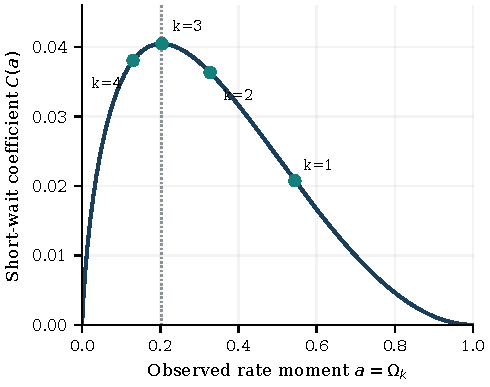
\includegraphics[width=\columnwidth]{refinement_20261112/figures/star_memory.pdf}
\caption{The exact short-wait coefficient and the four reconstructed
layer rates at $x=\log2/2$. The near optimum at three layers coexists with
the same uniform 16-mask equilibrium for every layer count.}
\label{fig:star-memory-12}
\end{figure}
